% Satu trace pemesanan janji temu Medikara+ ke rumah sakit Bandung, digambar sebagai
% diagram air terjun. Setiap batang adalah satu span; panjangnya sebanding dengan
% durasi. Garis putus-putus merah menandai batas tunggu aplikasi di ponsel pasien.
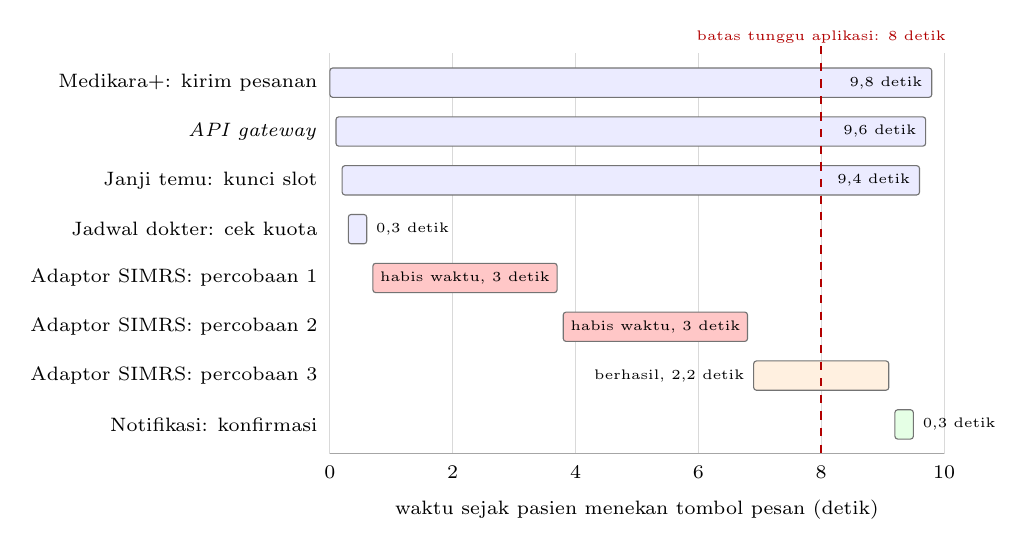
\begin{tikzpicture}[
  x=0.78cm, y=0.62cm,
  font=\scriptsize,
  execute at begin node={\hyphenpenalty=10000},
  nama/.style={anchor=east, inner sep=1pt},
  durasi/.style={font=\tiny, inner sep=1pt},
  batang/.style={draw=black!55, rounded corners=1pt},
  panah/.style={-{Stealth[length=2mm]}, thick}
]
  % Garis bantu dan sumbu waktu
  \foreach \t in {0, 2, 4, 6, 8, 10} {
    \draw[gray!30] (\t, 0.1) -- (\t, -8.1);
    \node[anchor=north] at (\t, -8.15) {\t};
  }
  \draw[gray!70] (0, -8.1) -- (10, -8.1);
  \node[anchor=north] at (5, -8.85)
    {waktu sejak pasien menekan tombol pesan (detik)};

  % Baris 1 sampai 3: span induk yang menunggu sampai seluruh langkah selesai
  \fill[blue!8, batang] (0.0, -0.2) rectangle (9.8, -0.8);
  \node[nama] at (-0.15, -0.5) {Medikara+: kirim pesanan};
  \node[durasi, anchor=east] at (9.7, -0.5) {9,8 detik};

  \fill[blue!8, batang] (0.1, -1.2) rectangle (9.7, -1.8);
  \node[nama] at (-0.15, -1.5) {\textit{API gateway}};
  \node[durasi, anchor=east] at (9.6, -1.5) {9,6 detik};

  \fill[blue!8, batang] (0.2, -2.2) rectangle (9.6, -2.8);
  \node[nama] at (-0.15, -2.5) {Janji temu: kunci slot};
  \node[durasi, anchor=east] at (9.5, -2.5) {9,4 detik};

  % Baris 4: cek kuota yang cepat
  \fill[blue!8, batang] (0.3, -3.2) rectangle (0.6, -3.8);
  \node[nama] at (-0.15, -3.5) {Jadwal dokter: cek kuota};
  \node[durasi, anchor=west] at (0.7, -3.5) {0,3 detik};

  % Baris 5 sampai 7: tiga percobaan ke adaptor SIMRS Bandung
  \fill[red!22, batang] (0.7, -4.2) rectangle (3.7, -4.8);
  \node[nama] at (-0.15, -4.5) {Adaptor SIMRS: percobaan 1};
  \node[durasi] at (2.2, -4.5) {habis waktu, 3 detik};

  \fill[red!22, batang] (3.8, -5.2) rectangle (6.8, -5.8);
  \node[nama] at (-0.15, -5.5) {Adaptor SIMRS: percobaan 2};
  \node[durasi] at (5.3, -5.5) {habis waktu, 3 detik};

  \fill[orange!12, batang] (6.9, -6.2) rectangle (9.1, -6.8);
  \node[nama] at (-0.15, -6.5) {Adaptor SIMRS: percobaan 3};
  \node[durasi, anchor=east] at (6.8, -6.5) {berhasil, 2,2 detik};

  % Baris 8: konfirmasi yang terkirim setelah aplikasi menyerah
  \fill[green!10, batang] (9.2, -7.2) rectangle (9.5, -7.8);
  \node[nama] at (-0.15, -7.5) {Notifikasi: konfirmasi};
  \node[durasi, anchor=west] at (9.6, -7.5) {0,3 detik};

  % Batas tunggu aplikasi di ponsel pasien
  \draw[red!70!black, dashed, thick] (8, 0.25) -- (8, -8.1);
  \node[durasi, anchor=south, text=red!70!black] at (8, 0.25)
    {batas tunggu aplikasi: 8 detik};
\end{tikzpicture}
